\section{Komponentenschnitt}\label{sec:komponentenschnitt}

\begin{figure}[H]
    \centering
    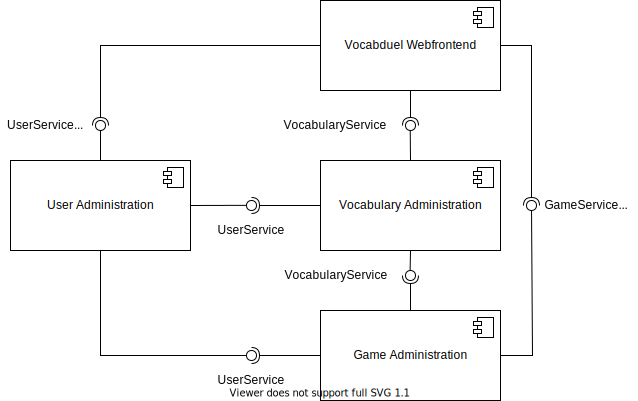
\includegraphics[width=0.8\textwidth]{components_diagram}
    \caption[]{Komponentenschnitt}
    \label{fig:komponenten-1}
\end{figure}

\subsection{Services}

Das Informationssystem lässt sich in die folgenden Services gruppieren:

\begin{outline}
    \1 \texttt{vocabulary\_administration}
    \1 \texttt{game\_administration}
    \1 \texttt{user\_administration}
\end{outline}

Das Modul \texttt{user\_administration} ist für das Nutzer-Management zuständig:
Es stellt wiederum zwei Services bereit: den \texttt{AuthService} für die Verwaltung von Zugangsdaten,
d.h.\ Passwörtern und JWT-Token, sowie den \texttt{UserService} zum Abfragen, Bearbeiten und Löschen
bestehender Nutzerdaten.

\texttt{vocabulary\_administration} ist für das Vokabel-Management zuständig:
Mithlife des \texttt{VocabularyService} wird der Zugriff sowie die Verwaltung von Vokabellisten bereitgestellt.

\texttt{game\_administration} ist für das Spiel-Management zuständig:
Durch die Bereitstellung des \texttt{GameService} wird eine Spielverwaltung zur Verfügung gestellt,
während der \texttt{ScoreService} für die Verwaltung von abgeschlossenen Spielen zuständig ist.

Alle dieser genannten Module existieren wiederum in drei Ausführungen:
\begin{outline}
    \1 Als Export-Schnittstellen, die von anderen Modulen genutzt werden können
    \1 Als tatsächliche Implementierungen, in denen die eigentliche Anwendungslogik implementiert ist und Datenbankzugriffe über DAOs erfolgen
    \1 Als Rest-Adapter, die zu ihrem jeweiligen Verantwortungsbereich eine REST-API bereitstellen
\end{outline}

\subsection{Konfigurationen und geteilte Module}\label{subsec:konfigurationen-und-geteilte-module}

Des Weiteren existieren folgende Module:

\begin{outline}
    \1 \texttt{configuration}/\texttt{configuration\_core}
    \1 \texttt{shared\_logic.rest}
    \1 \texttt{vocabduel\_ui}
\end{outline}

Zusätzlich existieren zwei Konfigurationskomponenten, wobei \texttt{configuration.rest} Spring RestEasy mit dem Angular Frontend beinhaltet und
\texttt{configuration} eine Starter-Datei (s.u.) zum Konsolen UI bereitstellt.
Beide Komponenten nutzen den über \texttt{configuration\_core} bereitgestellten Transaktionsmanager (Hibernate).
Auf diesem Weg ist eine strikte Trennung zwischen den beiden Konfigurationen möglich ohne aber mehrfache Transaktionsmanager definieren zu müssen.

Die Komponente \texttt{vocabduel\_ui} stellt das User Interface für die Configuration bereit, welches auf der Konsole ausgeführt wird.
Die Komponente \texttt{shared\_logic.rest} wird in der Rest-Schicht der Administrations-Komponenten genutzt, um RefreshToken
zur Web-Session und fehlende Daten beim API-Aufruf zu managen.


